	\section{Komunia Święta \textit{bardziej uroczysta}}
	
		\subsection{Komunia Święta dwójkami – bez obrusu komunijnego}
		
			\begin{itemize}
				\item Ministranci biorący udział w lucenarium wchodzą dwójkami do prezbiterium, tworząc w ten sposób naturalną „kolejkę”. Przed nimi do kolejki wchodzą akolici, trzymając w rękach patenę. Za nimi miejsce zajmuje ceremoniarz razem z turyferem lub innym ministrantem.
				\item Na znak ceremoniarza cała procesja komunijna najpierw przyklęka, a potem klęka na dwa kolana. Akolici wchodzą na najwyższy stopień ołtarza i przyjmują Komunię Świętą jako pierwsi.
				\item Akolici po przyjęciu Komunii Świętej na najwyższym stopniu ołtarza i przyklęknięciu zajmują miejsce przy celebransie z pateną i świeczką sanctusową.
				\item Każda para tuż przed przyjęciem Komunii Świętej przyklęka na podłodze, razem z parą poprzedzającą, która już Komunię przyjęła.
				\item Każda para po przyjęciu Komunii Świętej przyklęka, po czym odchodzi na stronę Ewangelii, w kierunku chóru.
			\end{itemize}
	
		\subsection{Śpiewana bardziej uroczysta – z obrusem}
		
			\begin{itemize}
				\item Podczas śpiewu \textit{Agnus Dei} 1.akolita bierze z kredencji obrus komunijny, razem z 2. akolitą klękają pośrodku, wchodzą na najwyższy stopień ołtarza i klęcząc przodem do siebie trzymają rozłożony obrus.
					\begin{figure}[h]
						\centering
						\includegraphics[width=0.5\linewidth]{komunia_1}
						\caption{Procesja do Komunii Św.}
						\label{fig:komunia_1}
					\end{figure}
				\item Ministranci biorący udział w lucenarium wchodzą dwójkami do prezbiterium, tworząc w ten sposób naturalną „kolejkę” do Komunii św. Przed nimi do kolejki wchodzą księża, klerycy i ceremoniarz, za nimi reszta ministrantów z chóru. 1Crm – zależnie od ilości duchownych i ministrantów może staje do komunii sam lub w parze.
				\item Ceremoniarz podaje patenę pierwszemu duchownemu przyjmującemu Komunię św., albo jeśli nie ma duchownych trzyma ją sam. Po przyjęciu Komunii	Św. Zajmuje miejsce przy celebransie, gdzie asystuje z pateną.
				\item 2Crm lub turyfer po przyjęciu Komunii św. zajmuje miejsce przy celebransie ze świeczką sanctusową.
					\begin{figure}[h]
						\centering
						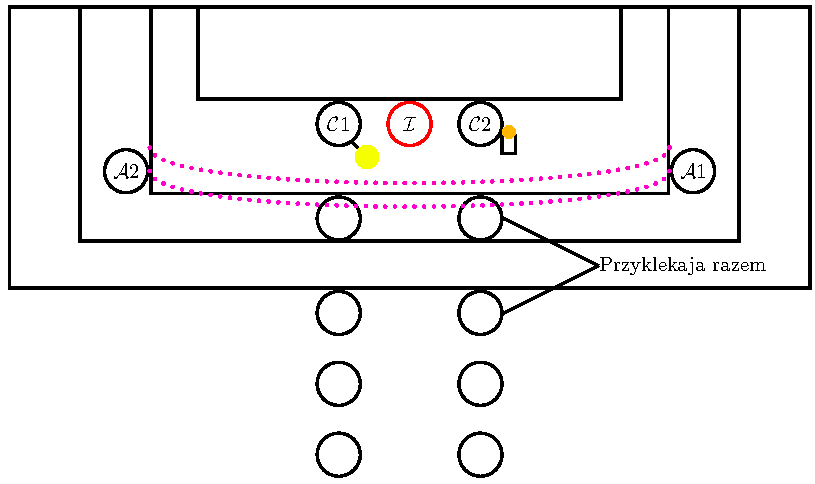
\includegraphics[width=0.5\linewidth]{komunia_2}
						\caption{W trakcie udzielania Komunii Św. ministrantom}
						\label{fig:komunia_2}
					\end{figure}
				\item Akolici trzymający obrus przyjmują Komunię św. razem z 1 Crm.
				\item Każda dwójka przystępująca do Komunii św. przyklęka jednocześnie z poprzedzającą parą, wchodzi na stopnie i klęka na dwa kolana. Po przyjęciu komunii znów przyklęka jednocześnie z parą stojącą za nimi. Ze stopni ołtarza schodzimy w lewo – do chóru.
				\item Po przyjęciu Komunii Św. Przez ministrantów akolici wstają i przechodzą do miejsca udzielania komunii wiernym. Z pateną i świeczką sanctusową asystują ceremoniarze.
					\begin{figure}[h]
						\centering
						\includegraphics[width=0.5\linewidth]{komunia_3}
						\caption{W trakcie udzielania Komunii Św. ludowi}
						\label{fig:komunia_3}
					\end{figure}
			\end{itemize}
		
		\clearpage
		
		\subsection{Msza solenna}
			
			\begin{itemize}
				\item Podczas śpiewu \textit{Agnus Dei} przekazywany jest znak pokoju – subdiakon przekazuje go duchownym w chórze i ceremoniarzowi.
				\item Ministranci biorący udział w lucenarium wchodzą dwójkami do prezbiterium, tworząc w ten sposób naturalną „kolejkę” do Komunii św. Zostawiają przed sobą miejsce dla duchownych, mających przyjąć Komunię. Za nimi ustawia się reszta ministrantów
			\end{itemize}
		
		\subsection{Komunia z obrusem na mszy solennej}
			
			\begin{itemize}
				\item Po ewentualnym. odebraniu znaku pokoju 1.akolita bierze z kredencji obrus komunijny, razem z 2. akolitą klękają pośrodku, wchodzą na najwyższy stopień ołtarza i klęcząc przodem do siebie trzymają rozłożony obrus.
				\item Porządek Komunii Św. (patrz obrazki przy mszy śpiewanej z obrusem)
					\begin{itemize}
						\item diakon i subdiakon
						\item kapłani, klerycy
						\item akolici trzymający obrus i 1Crm
						\item 2Crm i turyfer
						\item reszta ministrantów.
					\end{itemize}
				\item Jeśli diakon nie rozdaje komunii, razem z sudbiakonem asystują kapłanowi. Podąża za nimi 1 Crm ze świeczką sanctusową.
					\begin{figure}[h]
						\centering
						\includegraphics[width=0.5\linewidth]{komunia_3_uro}
						\caption{W trakcie udzielania Komunii Św. ludowi (diakon nie rozdaje)}
						\label{fig:komunia_3_uro}
					\end{figure}
				\item Jeśli diakon lub inny kapłan rozdaje komunię przy obrusie:
					\begin{itemize}
						\item celebransowi asystuje subdiakon z pateną
						\item diakonowi asystuje 2 Crm z pateną
						\item dwóch wyznaczonych ministrantów z chóru po przyjęciu Komunii zapala świeczki i przy udzielaniu komunii wiernym, klęczą ze świeczkami bo dwóch stronach obrusa.
					\end{itemize}
					\begin{figure}[ht]
						\centering
						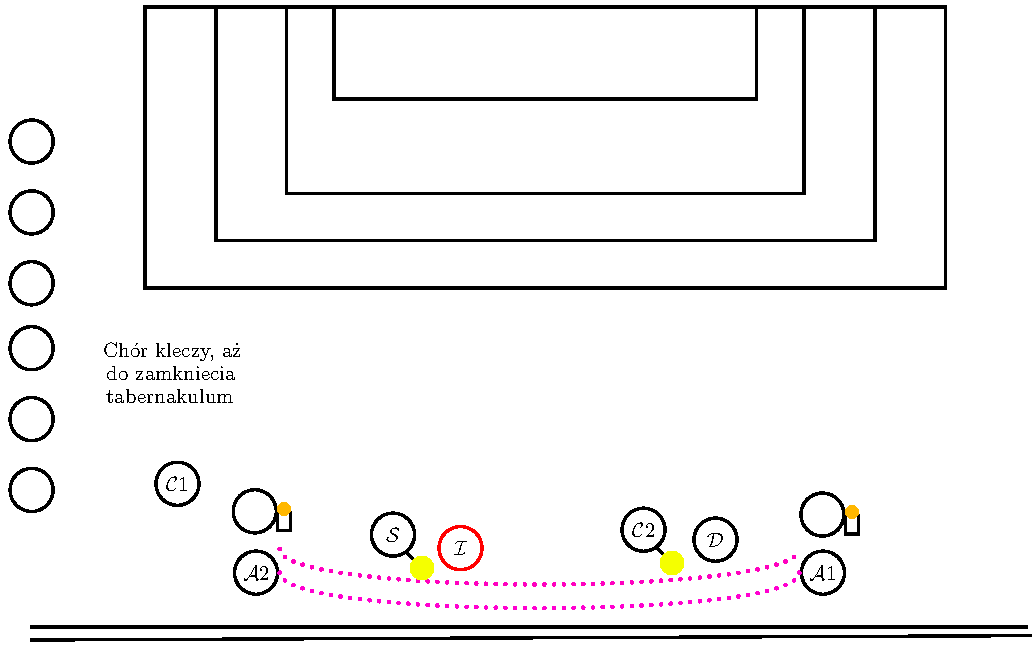
\includegraphics[width=0.5\linewidth]{komunia_3_uro_diak}
						\caption{W trakcie udzielania Komunii Św. ludowi (diakon rozdaje)}
						\label{fig:komunia_3_uro_1}
					\end{figure}
			\end{itemize}
    
    \subsection{Komunia na Mszy solennej lub śpiewanej bez obrusa}
    
			Jeśli diakon lub inny kapłan rozdaje Komunię św., ceremoniarz asystuje ze świeczką celebransowi, a akolici z pateną i świeczką asystują diakonowi.
			
			\begin{figure}[ht]
				\centering
				\includegraphics[width=0.5\linewidth]{komunia_1_uro_bez}
				\caption{W trakcie udzielania Komunii Św. ludowi (diakon rozdaje)}
				\label{fig:komunia_1_uro_bez}
			\end{figure}
		
			\begin{figure}[ht]
				\centering
				\includegraphics[width=0.5\linewidth]{komunia_3_uro_diak_bez}
				\caption{W trakcie udzielania Komunii Św. ludowi (diakon rozdaje)}
				\label{fig:komunia_3_uro_diak_bez}
			\end{figure}
	
	\clearpage
 